
\chapter{Qubits et états quantiques}
\label{sec:AmplProb}
\minitoc

\bigskip


Dans ce chapitre nous présentons le cadre général de la théorie quantique en
utilisant la puissante et élégante algèbre de Dirac. La \textbf{section
\ref{sec:Inter1Part}} est consacrée à la découverte de l'étrange monde quantique
à travers quelques expériences d'interférences à une particule. Ces expériences
montrent que l'intuition et le \emph{bon sens} hérités de la physique classique
sont inadaptés dans le monde quantique du fait de la nature fondamentalement
\textbf{probabiliste} ou \textbf{indéterministe} des phénomènes quantiques.
Cette nature impose l'introduction, à la \textbf{section \ref{sec:AmplProba}},
des concepts nouveaux et essentiels d'état quantique, d'amplitude de probabilité
ou amplitude de transition, de superposition d'état ou \textbf{qubit} et de
l'espace de Hilbert. Ces concepts ont été auparavant présenté de façon
\emph{mathématique} à la \textbf{section \ref{sec:qbit}}.

\section{Qubit ou bit quantique et espace de Hilbert}
\label{sec:qbit}

\subsection{Qubit ou bit quantique}

L'unité fondamentale de l'informatique classique est le bit (de l'anglais
\emph{binary digit}). Un bit peut prendre deux valeurs que l'on note
habituellement $0$ et $1$. Évidemment, ce choix de notation, complètement
arbitraire, n'est que la représentation symbolique du stockage du bit dans un
système à deux états. En effet, la valeur $0$ d'un bit peut être représentée
physiquement dans un ordinateur par un condensateur non chargé et la valeur $1$,
représentée par le même condensateur chargé (voir la figure
\ref{fig:CodageClas}). La différence entre les deux états (chargé et non chargé)
se traduit par le déplacement de plusieurs millions d'électrons. Ainsi, un bit
d'information classique implique environ $10^{9}$ électrons dans la mémoire vive
d'un ordinateur. Il s'agit donc d'un comportement \emph{collectif}.

\begin{figure}[ptbh]
\centering
\ifcase\msipdfoutput
  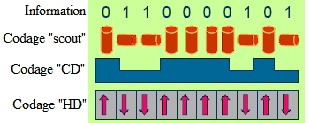
\includegraphics[scale=1]{graphics/CodageClas.jpg}
\else
  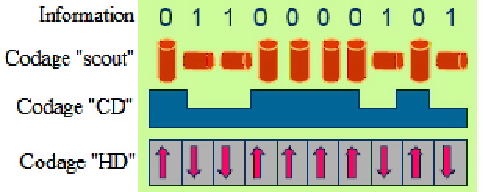
\includegraphics[scale=1]{graphics/CodageClas.pdf}
\fi
\caption{\textbf{Codage classique}. L'information, que l'on représente par les
\textbf{bits} $0$ et $1$, est toujours codée dans des systèmes physiques
bistables.}
\label{fig:CodageClas}%
\end{figure}

\begin{figure}[ptbh]
\centering
  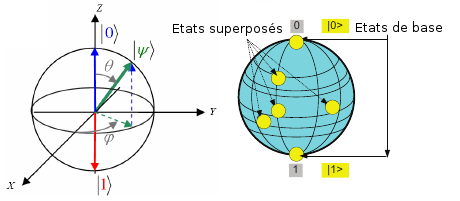
\includegraphics[scale=1]{graphics/SphereBloch.png}%
\caption{\textbf{Codage quantique.} Le qubit $\ket{\psi} =\alpha\ket{0}
+\beta\ket{1}$ (avec $\alpha=\cos\frac{\theta}{2},
\beta=e^{i\varphi}\sin\frac{\theta}{2}$ et $|\alpha|^{2}+|\beta|^{2}=1$), offre
une description différente des systèmes physiques. Les états binaires classiques
sont aux pôles de la sphère. Il opère dans un univers multidimensionnel, ces
états propres correspondant à la surface de la sphère, alors que les états
logiques classiques correspondent aux pôles de cette sphère.}
\label{fig:SphereBloch}
\end{figure}

L'unité fondamentale de l'information quantique est le bit quantique ou, plus
simplement, \textbf{qubit} (de l'anglais \emph{quantum bit}). Il est
superficiellement similaire au bit classique, mais comme nous le ferons, il est
fondamentalement différent et cette différence fondamentale permet le
traitement de l'information de façons nouvelles et très prometteuses.

Comme le bit, le qubit peut-être dans un des états $0$ ou $1$. Pour une raison
qu'on expliquera ci-dessous, on notera ces états $\ket{0}$ et $\ket{1}$ et on
lira \textbf{\emph{ket de 0}} et \textbf{\emph{ket de 1}}. Cette notation est
appelée \textbf{notation de Dirac} et représente un \emph{vecteur d'état} ou
un \emph{état} tout simplement.

A la différence du bit classique, le qubit peut-être \textbf{à la fois} dans
l'état $\ket{0}$ et  $\ket{1}$. On dit alors qu'il est dans \textbf{état
superposé} que l'on note
\begin{equation}
\ket{\psi}=\alpha\ket{0}+\beta\ket{1},
\end{equation}
où $\alpha$ et $\beta$ sont des nombres complexes qui vérifient
\begin{equation}
 |\alpha|^{2}+|\beta|^{2}=1,
\end{equation}
appelée \textbf{relation de complétude} ou \textbf{condition de normalisation}
du qubit. La figure \ref{fig:SphereBloch} donne une représentation du qubit sur
une sphère de Bloch.

Tant qu'on effectue aucune mesure ou alors tant que le qubit est isolé du monde
extérieur, il reste dans cet état superposé. Dès qu'une mesure est effectuée
ou dès que le qubit est en contact avec son environnement, il adopte un
comportement classique en prenant \textbf{soit} l'état $\ket{0}$, \textbf{soit}
l'état $\ket{1}$. Et les lois de la théorie quantique nous disent que

\colorbox[gray]{0.8}{
\parbox[c]{0.9\textwidth}{
\begin{itemize}
\item on trouve le qubit $\ket{\psi}$ dans l'état $\ket{0}$ avec la
\textbf{probabilité} $|\alpha|^{2}$;
\item on trouve le qubit $\ket{\psi}$ dans l'état $\ket{1}$ avec la
\textbf{probabilité} $|\beta|^{2}$.
\end{itemize}
}}

D'une manière générale, si un qubit est une superposition de $N$
états\footnote{Lorsqu'on a un état quantique de dimension $d\geq 3$ on parle de
\textbf{qudit}. Par exemple, pour $d=3$, on a un \textbf{qutrit} et  pour $d=4$
on a un \textbf{ququart}.} $\ket{i}$,
\begin{subequations}
 \begin{align}
\ket{\psi}=\sum_{i=0}^{N-1}\alpha_{i}\ket{i},
\end{align}
on a
\begin{align}
 \sum_{i=0}^{N-1}|\alpha_{i}|^{2}=|\alpha_{0}|^{2}+|\alpha_1|^{2}
+\cdots+|\alpha_{N-1}|^{2}=1.
\end{align}
\end{subequations}
Les coefficients $\alpha_{i}$ sont appelés \textbf{amplitudes de probabilité}.
Puisque ce sont des nombres complexes en général, on calcule les probabilités
$|\alpha_{i}|^{2}$ de la façon suivante,
\begin{equation}
 |\alpha_{i}|^{2}=\alpha_{i}^{*}\alpha_{i},
\end{equation}
où $\alpha_{i}^{*}$ est le complexe conjugué de $\alpha_{i}$.

La dichotomie qu'il y a entre le comportement du qubit quand il n'est pas
observé (ou lorsqu'il est isolé) et lorsqu'il est observé (ou en contact
avec l'environnement), est au cœur même de la théorie quantique.

\begin{figure}[ptbh]
 \centering
\includegraphics[scale=.65]{graphics/QubitAtom2Levels1.png}
\caption{Qubit représenté par deux états électroniques d'un atome [Après
Nielsen et Chuang\cite{MNIC2000}]}
 \label{fig:QubitAtom2Levels}
\end{figure}

Malgré son comportement étrange, le qubit existe réellement. En effet,
nombre de systèmes physiques peuvent être utilisés pour réaliser un qubit.
C'est le cas par exemple des deux états d'un électron orbitant autour du noyau
d'un atome qu'illustre la figure \ref{fig:QubitAtom2Levels}. Dans le modèle
de l'atome, un électron est soit dans un état fondamental soit dans un état
excité, que l'on peut représenter respectivement par $\ket{0}$ ou $\ket{1}$.
Lorsqu'on envoie un rayonnement électromagnétique avec une énergie appropriée,
il est possible de déplacer l'électron de l'état $\ket{0}$ vers $\ket{1}$ et
vice-versa. Mais il est encore plus intéressant d'éclairer l'atome avec un
rayonnement ayant une énergie telle que, l'électron initialement dans l'état
$\ket{0}$ se trouve à mi-chemin entre $\ket{0}$ et $\ket{1}$, dans l'état
\begin{equation}
 \ket{\psi}=\frac{1}{\sqrt{2}}(\ket{0}+\ket{1}).
\end{equation}

On retient que

\medskip
\colorbox[gray]{0.8}{
\parbox[c]{0.9\textwidth}{
\emph{La différence entre le bit classique et le bit quantique ou qubit se situe
au niveau de la description d'un système physique (ses propriétés), étant
entendu que l'\textbf{état} d'un système est l'ensemble des propriétés que le
système possède. Si on pose par exemple la question \textbf{est-il possible de
trouver la propriété $P$ du système lors d'une mesure?} La théorie classique
répond \textbf{NON} alors que la théorie quantique répond \textbf{OUI mais avec
une probabilité} $|\alpha|^{2}$ par exemple.}
}}


\begin{exercise}
For each of the following qubits, if a measurement is made, what is the
probability that we find the qubit in the state $\ket{0}$? What is the
probability that we find the qubit in the state $\ket{1}$?
\begin{enumerate}
 \item $\ket{\psi}=\frac{1}{\sqrt{3}}\ket{0}+\sqrt{\frac{2}{3}}\ket{1}$.
 \item $\ket{\psi}=\frac{i}{2}\ket{0}+\frac{\sqrt{3}}{2}\ket{1}$.
 \item $\ket{\psi}=\frac{1+i}{\sqrt{3}}\ket{0}-\frac{i}{\sqrt{3}}\ket{1}$.
\end{enumerate}
\end{exercise}

\begin{footnotesize}
\begin{solution}
 To find the probability that each qubit is found in the state $\ket{0}$ or the
state $\ket{1}$, we compute the modulus squared of the appropriate coefficient.
\begin{enumerate}
 \item The probability of finding $\ket{\psi}$ in the state $\ket{0}$ is
\begin{subequations}
\begin{align}
\left|\frac{1}{\sqrt{3}}\right|^{2}=\frac{1}{3},
\end{align}
whereas probability of finding $\ket{\psi}$ in the state $\ket{1}$ is
\begin{align}
 \left|\sqrt{\frac{2}{3}}\right|^{2}=\frac{2}{3}.
\end{align}
These probabilities verified
\begin{align}
 \sum_{i=0}^{1}|\alpha_{i}|^{2}=\frac{1}{3}+\frac{2}{3}=1.
\end{align}
\end{subequations}
  \item The next state has coefficients that are complex numbers. So that
the probability of finding $\ket{\psi}$ in the state $\ket{0}$ is
\begin{subequations}
\begin{align}
\left|\frac{i}{2}\right|^{2}=\left(\frac{i}{2}\right)^{*}\left(\frac{i}{2}
\right)=\left(-\frac{i}{2}\right)\left(\frac{i}{2}\right)=\frac{1}{4},
\end{align}
whereas probability of finding $\ket{\psi}$ in the state $\ket{1}$ is
\begin{align}
 \left|\frac{\sqrt{3}}{2}\right|^{2}=\frac{3}{4}.
\end{align}
Again, we check that the probabilities sum to $1$:
\begin{align}
 \sum_{i=0}^{1}|\alpha_{i}|^{2}=\frac{1}{4}+\frac{3}{4}=1.
\end{align}
\end{subequations}
  \item Finally, for the last state, the probability of finding $\ket{\psi}$ in
the state $\ket{0}$ is
\begin{subequations}
\begin{align}
\left|\frac{1+i}{\sqrt{3}}\right|^{2}=\left(\frac{1+i}{\sqrt{3}}
\right)^{*}\left(\frac{1+i}{\sqrt{3}}\right)=\left(\frac{1-i}{\sqrt{3}}
\right)\left(\frac{1+i}{\sqrt{3}}\right)=\frac{1-i+i+1}{3}=\frac{2}{3},
\end{align}
whereas probability of finding $\ket{\psi}$ in the state $\ket{1}$ is
\begin{align}
 \left|\frac{i}{\sqrt{3}}\right|^{2}=\left(\frac{i}{\sqrt{3}}
\right)^{*}\left(\frac{ i}{\sqrt{3}}\right)=\left(-\frac{i}{\sqrt{3}}
\right)\left(\frac{ i}{\sqrt{3}}\right)=\frac{1}{3} .
\end{align}
Again, these probabilities sum to $1$:
\begin{align}
 \sum_{i=0}^{1}|\alpha_{i}|^{2}=\frac{2}{3}+\frac{1}{3}=1.
\end{align}
\end{subequations}

\end{enumerate}

\textbf{\emph{Pas du tout compliqué n'est-ce pas?}}
\end{solution}
\end{footnotesize}

\subsection{Espace de Hilbert}
\label{sec:EH}

L'espace mathématique où ont lieu les calculs quantiques est l'\textbf{espace de
Hilbert} $\mathcal{H}$, qui est un espace Euclidien complexe, muni d'un produit
scalaire. C'est un espace de dimension infinie, mais nous nous limiterons dans
cette section au cas de la dimension finie.
\begin{enumerate}
\item Le \textbf{ket} $\ket{i}$ est un vecteur de l'espace des états ou
\textbf{espace de Hilbert }$\mathcal{H}$;

\item Le \textbf{bra} $\bra{f}$ est un vecteur de l'espace dual
$\mathcal{H}^{\ast}$, autrement, c'est le \textbf{conjugué hermitien} du
$\ket{f}$,
\begin{equation}
 (\ket{f})^{\dag}=\bra{f}.
\end{equation}
\end{enumerate}

Il existe une correspondance biunivoque entre les vecteurs de ces deux
espaces. On utilise le même symbole pour représenter un vecteur de l'un de ces
espaces et celui qui lui correspond dans l'autre espace. Ainsi, le vecteur de
l'espace des états correspondant au bra $\bra{f}$ est le ket $\ket{f}$.

\subsubsection{Base hilbertienne}

\medskip\colorbox[gray]{0.8}{
\parbox[c]{0.9\textwidth}{
\begin{definition}
L'ensemble $\mathcal{B}=\{\ket{i}\}$ est \textbf{une base hilbertienne}, si
\begin{equation}
\langle i\ket{j} =\delta_{ij}=\begin{cases}
1 & \text{si }i=j,\\
0 & \text{sinon,}
\end{cases}
\label{eq:dij}
\end{equation}
et
\begin{equation}
\sum_{i\in\mathcal{B}}\ket{i}\bra{i}=\mathbf{1}.
\label{eq:RF}
\end{equation}
La \textbf{relation de fermeture} (\ref{eq:RF}) permet la projection d'un
vecteur d'état dans la base $\mathcal{B}$.
\end{definition}
}}

Ainsi, le ket $\ket{y} $ se développe dans la base hilbertienne $\mathcal{B}$,
compte tenu de la relation de fermeture (\ref{eq:RF}), sous la forme%
\begin{subequations}
\begin{align}
\ket{y} =\sum_{i\in B}\ket{i} \langle i\ket{y} =\alpha_{i}\ket{i},
\end{align}
\label{eq:XY}%
avec%
\begin{align}
\alpha_{i}=\langle i\ket{y},
\end{align}
\end{subequations}
considérée ici comme la \textbf{coordonnée} ou la \textbf{projection} ou plus
précisément \textbf{l'amplitude de probabilité de projection} de $\ket{y}$
suivant $\ket{i}$.

Puisque le bra $\bra{x}$ appartient à \textbf{l'espace dual}
$\mathcal{H}^{\ast}$, on a la correspondance antilinéaire \textbf{ket}
$\rightarrow$\textbf{bra}:
\begin{subequations}%
\begin{align}
\lambda\ket{\psi}  &  \longrightarrow\lambda^{\ast}\bra{\psi},\\
\lambda_1\ket{\psi_1}+\lambda_2\ket{\psi_2}&
\longrightarrow\lambda_1^{\ast}\bra{\psi}_1+\lambda_2^{\ast}
\bra{\psi_2}.
\end{align}%
\end{subequations}%
Par suite,
\begin{equation}
\bra{x} =\sum_{i\in B}\langle x\ket{i}\bra{i} =\sum_{i\in B}\langle i\ket{x}
^{\ast}\bra{i} =\alpha_{i}^{\ast}\bra{i}.
\end{equation}
C'est ainsi que, dans base $\{\ket{i}\}$, les vecteurs d'états sont représentés
dans $\mathcal{H}$ par des nombres, valeurs des composantes ou amplitudes de
transition ou de projection:
\begin{subequations}%
\begin{align}
\ket{\psi} &  =\sum_{i}\ket{i}\langle i\ket{\psi}=\sum_{i}\alpha_{i}\ket{i}
\text{ avec }\langle i\ket{\psi} =\alpha_{i}\Rightarrow\ket{\psi} =
\begin{pmatrix}
\alpha_1\\
\alpha_2\\
\vdots\\
\alpha_{i}\\
\vdots
\end{pmatrix},\\
\bra{\psi} &  =\sum_{i}\langle\psi\ket{i}\bra{i}=\sum_{i}\bra{i}
\alpha_{i}^{\ast}\text{ avec }\bra{\psi}i\rangle=\alpha_{i}^{\ast}
\Rightarrow\bra{\psi}=(\alpha_1^{\ast},\alpha_2^{\ast},\cdots,\alpha_{i}^{
\ast},\cdots).
\end{align}%
\end{subequations}%

Si un vecteur $\ket{\varphi}$ se décompose sur la base $\{\ket{i}\}$ suivant
\begin{equation}
\ket{\varphi} =\sum_{i}\beta_{i}\ket{i},
\end{equation}
alors, en utilisant (\ref{eq:dij})%
\begin{equation}
\langle\psi\ket{\varphi} =\sum_{i,j=1}\langle\psi\ket{i}\bra{i}
j\rangle\langle j\ket{\varphi}=\sum_{i}\alpha_{i}^{\ast}\beta_{i}.
\label{eq:XY2}
\end{equation}

La notion d'état de la base hilbertienne peut être très bien comprise à
travers l'analogie avec l'espace $\mathcal{V}$ des vecteurs réels
tridimensionnels.

Considérons les vecteurs de base de $\mathcal{V}$%
\begin{equation}
\bls{e}_1=\begin{pmatrix}1\\0\\0\end{pmatrix},\ \bls{e}_2=\begin{pmatrix}
0\\1\\0\end{pmatrix},\ \bls{e}_{3}=\begin{pmatrix}0\\0\\1\end{pmatrix},
\end{equation}
et deux vecteurs de $\mathcal{V}$%
\begin{equation}
\bls{A}=\begin{pmatrix}
a_1\\
a_2\\
a_{3}\end{pmatrix},\ \bls{B}=\begin{pmatrix}
b_1\\
b_2\\
b_{3}\end{pmatrix}.
\end{equation}
Le vecteur
\begin{equation}
\bls{B}=\sum_{i=1}^{3}\bls{e}_{i}(\bls{e}_{i}
\cdot\bls{B})=\sum_{i=1}^{3}\bls{e}_{i}b_{i}=
b_1\bls{e}_1+b_2\bls{e}_2+b_{3}\bls{e}_{3}.
\label{eq:B}%
\end{equation}
qui apparaît comme la somme de ces composantes ou projections sur les vecteurs
de base, est l'analogue de la relation (\ref{eq:XY}).

L'analogue de la relation (\ref{eq:XY2}) est
\begin{equation}%
\begin{split}
\bls{A}\cdot\bls{B}  &  =\sum_{i=1}^{3}(\bls{A}\cdot\bls{e}_{i})
(\bls{e}_{i}\cdot\bls{B})\\
& =(\bls{A}\cdot\bls{e}_1)(\bls{e}_1\cdot\bls{B})
+(\bls{A}\cdot\bls{e}_2)(\bls{e}_2\cdot\bls{B})
+(\bls{A}\cdot\bls{e}_{3})(\bls{e}_{3}\cdot\bls{B})
\\
&  =a_1b_1+a_2b_2+a_{3}b_{3}.
\label{eq:AB2}%
\end{split}%
\end{equation}%
On note que les vecteurs $\bls{A}$ et $\bls{B}$ correspondent aux deux vecteurs
états $\ket{\psi} $ et $\ket{\varphi} $ et l'ensemble des vecteurs de base
correspondent à l'ensemble des vecteurs d'états de la base hilbertienne.

\begin{example}
Dans la base $\{\ket{+},\ket{-}\}$, l'état superposé $\ket{\psi}
=\frac{1}{\sqrt{2}}(\ket{+}+\ket{-})$ a pour composantes
\begin{equation}
\ket{\psi} =\frac{1}{\sqrt{2}}\left(\begin{pmatrix}
1\\
0
\end{pmatrix}+\begin{pmatrix}
0\\
1
\end{pmatrix}\right)=\frac{1}{\sqrt{2}}\begin{pmatrix}
1\\
1
\end{pmatrix}.
\end{equation}
\end{example}

\begin{example}
Soit un système quantique décrit dans la base d'états $\{\ket{a},\ket{b},\ket{c}
\}$. Dans cette représentation, les états $\ket{\psi} $ et $\ket{\varphi}$ ont
les amplitudes
\begin{subequations}%
\begin{align}
\langle a\ket{\psi}  &  =\frac{1}{\sqrt{3}},~\langle b\ket{\psi} =0,~\langle
c\ket{\psi}=i\sqrt{\frac{2}{3}},\\
\langle a\ket{\varphi} &  =\frac{1+i}{\sqrt{3}},~\langle b\ket{\varphi}
=\frac{1}{\sqrt{6}},~\langle c\ket{\varphi}=\frac{1}{\sqrt{6}}.
\end{align}
\end{subequations}%
La probabilité de trouver le système dans l'état $\ket{\varphi}$ alors qu'il se
trouvait initialement dans l'état $\ket{\psi}$ est
\begin{equation}%
\mathcal{P}_{\varphi\psi} =|\langle\varphi\ket{\psi}|^{2}=\left|
\sum_{i}\langle\varphi\ket{i}\langle i\ket{\psi}\right|^{2}=\left|
\frac{1\times(1-i)}{3}+0+i\sqrt{\frac{2}{3\times6}}\right|^{2}=\left|
\frac{1}{3}\right|^{2}=\frac{1}{9}.
\end{equation}%
Il est facile de vérifier que $\mathcal{P}_{\psi\varphi} =|\frac{1}{3}|^{2}
=\frac{1}{9}$.
\end{example}

\begin{exercise}
 Two vectors in $\mathbb{C}^{3}$ are given by $\ket{a}=\begin{pmatrix}
-2\\
4i\\
1
\end{pmatrix}$ and $\ket{b}=\begin{pmatrix}
1\\
0\\
i
\end{pmatrix}$.

Find
\begin{enumerate}
 \item $\bra{a}$, $\bra{b}$.
 \item $\langle a\ket{b}$, $\langle b\ket{a}$.
 \item $\ket{c}=\ket{a}+2\ket{b}$, $\langle c\ket{a}$.
\end{enumerate}
\end{exercise}

\begin{footnotesize}
\begin{solution}
 \begin{enumerate}
  \item The Hermitian conjugate is the complex conjugate of the transpose. Then,
\begin{subequations}
\begin{align}
 \bra{a}=(\ket{a})^{\dag}=(\ket{a}^{t})^{*}=(-2\quad-4i\quad 1),\\
 \bra{b}=(\ket{b})^{\dag}=(\ket{b}^{t})^{*}=(1\quad0\quad-i).
\end{align}
\end{subequations}
  \item From (\ref{eq:XY2}), the probability amplitude
\begin{subequations}
\begin{align}
 \langle a\ket{b}=(-2\quad-4i\quad 1)\begin{pmatrix}
1\\
0\\
i
\end{pmatrix}=-2+0+i=-2+i.
\end{align}
As $\langle a\ket{b}=\langle b\ket{a}^{*}$, we should find $\langle
b\ket{a}=-2-i$. We verify this with an explicit calculation
\begin{align}
 \langle b\ket{a}=(1\quad0\quad-i)\begin{pmatrix}
-2\\
4i\\
1
\end{pmatrix}=-2+0-i=-2-i.
\end{align}
\end{subequations}
 \item We apply the rules of vector addition and scalar multiplication to
obtain
\begin{subequations}
\begin{align}
 \ket{c}=\ket{a}+2\ket{b}=\begin{pmatrix}
-2\\
4i\\
1
\end{pmatrix}+2\begin{pmatrix}
1\\
0\\
i
\end{pmatrix}=\begin{pmatrix}
-2+21\\
4i+0\\
1+2i
\end{pmatrix}=\begin{pmatrix}
0\\
4i\\
1+2i
\end{pmatrix}
\end{align}
Therefore
\begin{align}
 (0\quad-4i\quad1-2i)\begin{pmatrix}
-2\\
4i\\
1
\end{pmatrix}=0+16+1-2i=17-2i.
\end{align}

\end{subequations}
 \end{enumerate}
\textbf{\emph{Aussi simple que ce qu'on apprend au Secondaire n'est-ce pas?}}
\end{solution}
\end{footnotesize}

\subsubsection{Produit scalaire}

Si on a
\begin{equation}
 \langle x\ket{y}=0,
\end{equation}
alors $\ket{x}$ et $\ket{y}$ sont \textbf{orthogonaux}. La symétrie hermitienne
du produit scalaire
\begin{equation}
 \langle x\ket{y}^{*}=\langle y\ket{x},
\end{equation}
implique que $\langle y\ket{y} $ est \emph{un nombre réel défini positif}%
\begin{subequations}
\begin{align}
\langle y\ket{y} \leq 0,
\end{align}
et
\begin{align}
\langle y\ket{y} =0\Rightarrow\ket{y} =0.
\end{align}
\end{subequations}

La \textbf{norme} d'un vecteur d'état $\ket{y} $ est définie par%
\begin{equation}
\|\ket{y}\| =\sqrt{\langle y\ket{y}}.
\end{equation}

Lorsque
\begin{equation}
 \langle x\ket{x}=1,
\end{equation}
on dit que le vecteur d'état $\ket{x}$ est \textbf{normalisé}.

Si chaque élément d'une base est normalisé et que les éléments de la base sont
orthogonaux les uns par rapport aux autres, on dit que la base est
\textbf{orthonormée}. C'est par exemple le cas de la base $\{\ket{+},\ket{-}\}$
avec
\begin{equation}
 \ket{+}=\frac{1}{\sqrt{2}}\binom{1}{1} ,\;
 \ket{+}=\frac{1}{\sqrt{2}}\binom{1}{-1}.
\end{equation} '
Une des propriétés importantes du produit scalaire est l'\emph{inégalité de
Cauchy-Schwarz}%
\begin{equation}
|\langle x\ket{y}|^{2}\leq\langle x\ket{x}\langle y\ket{y}
=\|\ket{x}\|^{2}\|\ket{y}\|^{2}.
\end{equation}

Maintenant que nous sommes un tout peu outillé en manipulations
mathématiques du qubit, des amplitudes de probabilités, des
probabilités, essayons de mieux les comprendre physiquement.

\section{Phénomènes quantiques: Interférence à une particule}

\label{sec:Inter1Part}

Afin de mettre en évidence l'étrange comportement des qubits, quelques
expériences ont été réalisées avec des objets quantiques (photons, électrons,
neutrons, atomes, molécules) isolées, ce qui écarte l'hypothèse des effets
collectifs\footnote{Mécanisme au terme duquel le sort d'un objet quantique
conditionnerait celui du suivant.}.
\bigskip

\emph{Rendons-nous donc au laboratoire!!}

\subsection{Fentes d'Young}

Commençons par le dispositif des fentes d'Young de la figure \ref{fig:DispYoung}
qui nous est très familier. La source $S$ émet un faisceau lumineux et le
détecteur mesure l'intensité lumineuse pour différentes positions de $x$. Si une
seule fente est ouverte, l'intensité est maximale à la position $x$ alignée
horizontalement sur la fente $F_1$. Lorsqu'on éloigne le détecteur de cette
position $x$, l'intensité diminue progressivement et devient nulle. Cependant,
lorsque les deux fentes sont ouvertes, la figure des intensités n'est pas
\textit{la somme} des deux figures d'intensité des fentes individuelles
ouvertes, mais plutôt une figure d'interférence: \textit{on observe au détecteur
une alternance de franges brillantes et de franges sombres} (voir la figure
\ref{fig:InterfLum}). Il y a donc interférence entre les faisceaux lumineux
provenant des deux fentes.

\begin{figure}[tbhp]
\begin{minipage}[c]{.48\linewidth}
\centering
\ifcase\msipdfoutput
	\includegraphics[scale=1]{graphics/DispYoung.eps}%
\else
	\includegraphics[scale=1]{graphics/DispYoung.pdf}%
\fi
\caption{Dispositif des fentes de Young}
\label{fig:DispYoung}%
\end{minipage} \hfill\begin{minipage}[c]{.48\linewidth}
\centering
\ifcase\msipdfoutput
	\includegraphics[scale=1]{graphics/InterfLum.eps}%
\else
	\includegraphics[scale=1]{graphics/InterfLum.jpg}%
\fi
\caption{Interférence lumineuse lorsque les deux fentes sont ouvertes. On a
une alternance de franges brillantes et de franges sombres.}%
\label{fig:InterfLum}%
\end{minipage}
\end{figure}

Utilisons maintenant un dispositif spécial dont la source $S$ ne produit que des 
électrons uniques qui sont dirigés vers les fentes $F_1$ et $F_2$. L'électron a 
une charge bien déterminée et la proposition \emph{un seul électron est bien 
passé soit par $F_1$, soit par $F_2$} est bien décidable (deux \textbf{chemins 
possibles}). Chaque électron est capté en un \emph{point bien précis} du 
détecteur comme on peut le voir sur la figure \ref{fig:InterfPhotons} (a). Ces 
points d'impact sont cependant \textbf{aléatoires}: les différents électrons 
indépendants préparés dans les \emph{mêmes} conditions ont des impacts 
\emph{différents}. Ce qui est en contradiction avec le 
\textbf{\emph{déterminisme}} classique qui veut à des \emph{conditions initiales 
identiques}, correspondent des \emph{conditions finales identiques}.

\begin{figure}[htbp]
\centering
\ifcase\msipdfoutput
  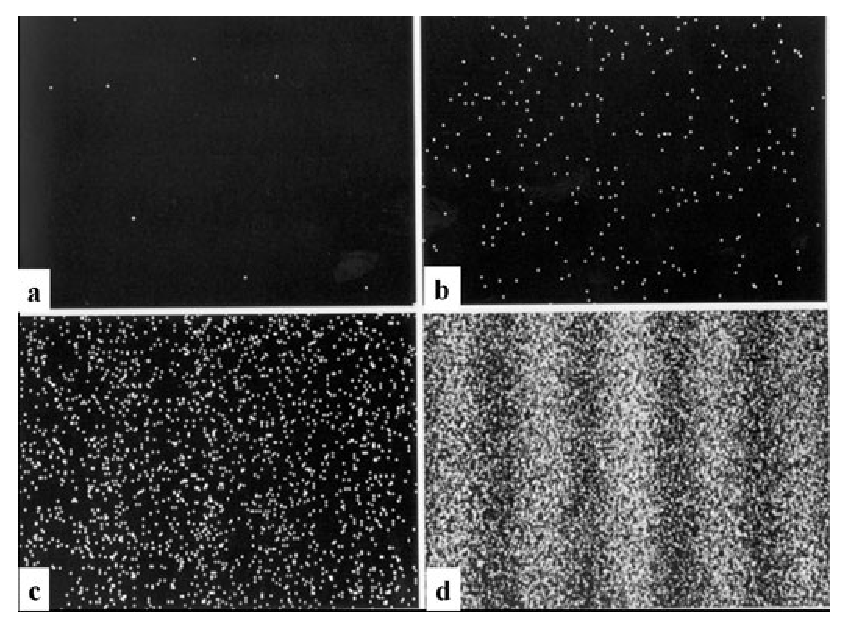
\includegraphics[scale=1]{graphics/InterfPhotons.eps}%
\else
  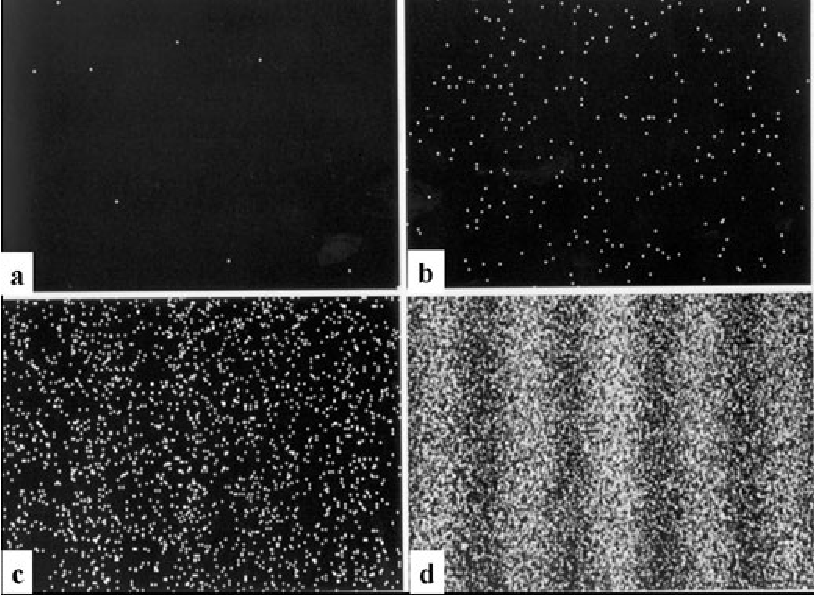
\includegraphics[scale=1]{graphics/InterfPhotons.pdf}%
\fi
\caption{Figures d'interférence obtenues avec des électrons uniques. Le nombre
d'électrons sur le détecteur augmente au cours du temps. Le temps d'exposition
entre la figure (a) et la figure (d) est multiplié par $20$. (a) 8 électrons;
(b) 270 électrons; (c) 2000 électrons; (d) 6000 électrons. [D'après Hitachi
Advanced Research Laboratory, Saitama, Japan].}%
\label{fig:InterfPhotons}%
\end{figure}

Au bout \emph{d'un temps suffisamment long}, on observe avec surprise que les
impacts des électrons forment une figure d'interférence comme illustrée par la
figure \ref{fig:InterfPhotons} (d). Ce résultat est surprenant en ce sens que
l'électron est un \textbf{corpuscule}. Or nous savons qu'une onde emplit tout
l'espace! Les électrons sont uns et \textbf{indivisibles}, donc il n'y a pas de
fragmentation d'un quantum d'énergie $\hbar\omega$. D'après Paul Dirac,
\textbf{chaque électron interfère avec lui-même} comme une onde\footnote{En
fait, avant la mesure, l'électron est dans une \textbf{superposition d'états},
et c'est chacun de ces états qui a interféré avec les autres.}. Il y a donc
antinomie: \emph{les concepts classiques d'onde et de corpuscules semblent ne
plus être valables pour les objets quantiques.}

Lorsqu'on réalise une autre expérience où le chemin emprunté par l'électron est
\textbf{discernable}, $F_1$ ouvert seul ou $F_2$ ouvert seul, on n'observe
pas de figure d'interférence, mais plutôt des impacts distribués autour des
sorties $F_1$ ou $F_2$. La somme de ces deux distributions distinctes ne
ressemble en rien la figure obtenue quand les deux fentes sont ouvertes. On ne
peut donc analyser le phénomène d'interférence des électrons uniques en termes
de probabilité classique: \textbf{\emph{lorsqu'à la même issue correspondent des
processus indépendants différents, la probabilité de cette issue n'est pas la
somme des probabilités individuelles}}.

\subsection{Interférométrie de Mach Zehnder}
\label{sec:InterfMZ}

Afin de mieux analyser le comportement des objets quantiques, examinons, après
V. Scarani\cite{VSC2004}, les expériences qui mènent à l'interférométrie de Mach
Zehnder. On a (voir les figures \ref{fig:MZ1}-\ref{fig:MZ4}):
\begin{itemize}
\item une \emph{source} qui envoie des objets quantiques isolés, un à un, l'un
après l'autre;

\item des \emph{séparateurs} qui sont des miroirs semi-transparents;

 \item et des \emph{détecteurs}, dispositifs de mesure permettant de compter les
objets quantiques.
\end{itemize}

\begin{figure}[ptbh]
\begin{minipage}[c]{.48\linewidth}
\centering
\ifcase\msipdfoutput
	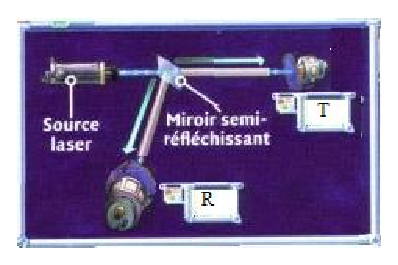
\includegraphics[scale=1]{graphics/MZ1.eps}%
\else
	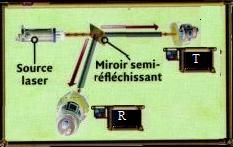
\includegraphics[scale=1]{graphics/MZ1.jpg}%
\fi
\caption{\emph{\textbf{Expérience MZ1:}} Montage à $2$ chemins ou fonctionnement
d'un miroir semi-transparent.}
\label{fig:MZ1}%
\end{minipage} \hfill\begin{minipage}[c]{.48\linewidth}
\centering
\ifcase\msipdfoutput
	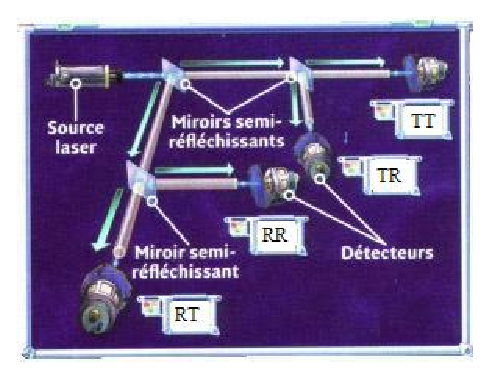
\includegraphics[scale=.9]{graphics/MZ2.eps}%
\else
	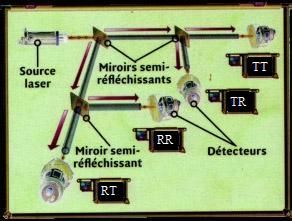
\includegraphics[scale=.9]{graphics/MZ2.jpg}%
\fi
\caption{\emph{\textbf{Expérience MZ2:}} Montage à
$4$ chemins avec $3$ miroir semi-transparents.}%
\label{fig:MZ2}%
\end{minipage}
\end{figure}

\subsection{Expérience MZ1}

Figure \ref{fig:MZ1}: Les objets quantiques arrivent individuellement sur le
séparateur et on compte combien d'entre eux sont réfléchis (R), et combien sont
transmis (T). Après le passage d'un grand nombre d'objets quantiques, on fait
les deux observations suivantes:

\begin{enumerate}
\item Les deux détecteurs ne s'activent jamais au même instant, donc
l'objet est \textbf{indivisible}, \emph{il est soit réfléchi, soit transmis}
(deux \textbf{chemins} possibles);

\item On dénombre la moitié des objets en R et l'autre en T, donc \emph{la
probabilité pour qu'un objet quantique soit réfléchi est la même qu'il soit
transmis} et les deux probabilités sont $50\%$.
\end{enumerate}

\subsection{Expérience MZ2}

Il y a lieu de se poser la question de savoir si en sortant de la source,
chaque objet n'a pas une \emph{instruction} lui permettant, chaque fois qu'il
rencontre un séparateur, d'être soit seulement réfléchie, soit seulement
transmis?

Afin d'élucider cela, à chaque sortie du premier séparateur, on place un autre
séparateur et on obtient \emph{quatre} chemins possibles (figure \ref{fig:MZ2}
): l'objet quantique peut être réfléchi deux fois (RR), réfléchi puis transmis
(RT), transmis puis réfléchi (TR) ou transmis deux fois (TT).

Si chaque objet avait une \emph{instruction} lui permettant, chaque fois qu'il
rencontre un séparateur, d'être soit seulement réfléchie, soit seulement
transmis, alors après le passage d'un grand nombre d'objets quantiques,
on observerait $50\%$ des objets en RR et $50\%$ des objets en TT, et rien en
RT\ ou TR.

Mais on observe qu'à chaque sortie, on a $25\%$ d'objets à chaque sortie.

\subsection{Expérience MZ3}

Figure \ref{fig:MZ3}: On a maintenant un interféromètre de Mach Zehnder: à
chaque sortie du premier séparateur, on place maintenant un miroir parfait qui
réfléchi tous les objets, les orientant vers un deuxième séparateur. Ainsi, une
des sorties du deuxième séparateur correspond aux chemins RT ou TR, l'autre aux
chemins RR ou TT. On a donc a nouveau quatre chemins possibles, de longueur
égale.

En vertu de la deuxième expérience, à la sortie RT ou TR, on observera
$25\%+25\%=50\%$ d'objets quantiques, et à la sortie RR ou TT, $50\%$ d'objets
quantiques.

Cependant, on observe que \emph{\textbf{tous les objets quantiques se trouvent
à la sortie RT ou TR}}: \textbf{le chemin RT est indiscernable du chemin TR}
après détection. \emph{On ne peut savoir quel chemin l'objet quantique détecté a
pris!}

On dit qu'il y a une \emph{\textbf{interférence constructive}} à la sortie RT
ou TR et une \emph{\textbf{interférence destructive}} à la sortie TT ou RR.
Puisqu'il y a une seule particule à la fois, on parle \textbf{d'interférence à
une particule}. Concrètement, un pic d'intensité sur une des sorties
correspond à un creux à l'autre sortie et inversement.

\medskip
\colorbox[gray]{0.8}{
\parbox[c]{0.9\textwidth}{
\emph{Le hasard quantique est vraiment étrange: lorsqu'on assemble d'une
certaine manière deux diviseurs de faisceau ou beam-splitters (générateurs de
hasard), on retrouve la certitude!}
}}
\medskip

Posons-nous les deux questions suivantes qui admettent les réponses \emph{oui}
ou \emph{non}:

\begin{enumerate}
\item[\textbf{Q1:}] l'objet quantique a-t-il pris le chemin T après le premier
séparateur?

\item[\textbf{Q2:}] l'objet quantique est-il détecté à la sortie RT ou TR?
\end{enumerate}

Dans la configuration de notre expérience MZ3, Q2 est toujours \emph{oui},
mais ne pouvons pas répondre à Q1.

Si on modifie l'expérience en insérant des détecteurs aux chemins R et T après
le premier séparateur, de sorte à pouvoir répondre à Q1, alors la réponse à la
question Q2 est modifiée. Seule la moitié des objets quantiques donneront la
réponse \emph{oui}, conformément à l'expérience MZ1. Donc si l'objet quantique
laisse une \emph{trace} de son passage, on observe pas d'interférence.

\medskip
\colorbox[gray]{0.8}{
\parbox[c]{0.9\textwidth}{
\emph{Il est donc impossible de savoir par quel chemin est passé l'objet
quantique et observer les interférences.} C'est le paradoxe connu sous le nom
du \emph{\textbf{chat de Schrödinger}}.
}}

\begin{figure}[ptbh]
\begin{minipage}[c]{.48\linewidth}
\centering
\ifcase\msipdfoutput
	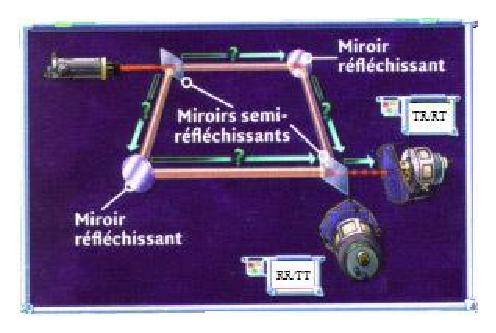
\includegraphics[scale=1]{graphics/MZ3.eps}%
\else
	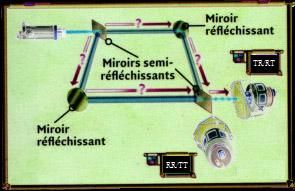
\includegraphics[scale=1]{graphics/MZ3.jpg}%
\fi
\caption{\emph{\textbf{Expérience MZ3:}} Interféromètre de Mach Zehnder
équilibré. \emph{\textbf{Les
chemins sont indiscernables.}}}
\label{fig:MZ3}%
\end{minipage} \hfill\begin{minipage}[c]{.48\linewidth}
\centering
\ifcase\msipdfoutput
	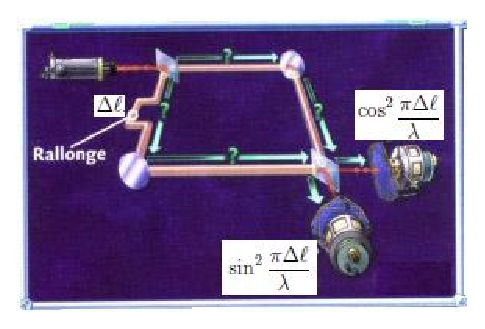
\includegraphics[scale=1]{graphics/MZ4.eps}%
\else
	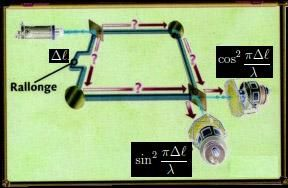
\includegraphics[scale=1]{graphics/MZ4.jpg}%
\fi
\caption{\emph{\textbf{Expérience MZ4:}} Interféromètre de Mach Zehnder
déséquilibré.
\emph{\textbf{Les chemins sont discernables et l'objet quantique explore tous
les chemins
possibles.}}}%
\label{fig:MZ4}%
\end{minipage}
\end{figure}

\subsection{Expérience MZ4}

Figure \ref{fig:MZ4}: On modifie la longueur des chemins RT ou TR, en y
introduisant par exemple une longueur supplémentaire $\Delta\ell$. On constate
que les probabilités de détection des objets quantiques aux sorties (RT ou TR)
et (RR ou TT) sont respectivement%
\begin{equation}
\cos^{2}\frac{\varphi}{2}\text{ et }\sin^{2}\frac{\varphi}{2},\ \varphi
=2\pi\frac{\Delta\ell}{\lambda}.
\end{equation}
Ainsi, lorsque par exemple,

\begin{itemize}
\item $\Delta\ell=\lambda$ (lame d'onde), tous les objets quantiques sont
détectés à la
sortie RT ou TR.

\item $\Delta\ell=\frac{\lambda}{2}$ (lame demi-d'onde), tous les objets
quantiques sont détectés
à la sortie RR ou TT;

\item $\Delta\ell=\frac{\lambda}{4}$ (lame quart-d'onde), une moitié des objets
quantiques est détectés à la
sortie RR ou TT et l'autre moitié à la sortie RT ou TR;

\end{itemize}

\medskip
\colorbox[gray]{0.8}{
\parbox[c]{0.9\textwidth}{
\emph{Donc, lorsqu'on modifie un seul des deux chemins, on modifie le
comportement des tous les objets quantiques.}
}}
\medskip

Comme on peut le voir sur les figures d'interférences \ref{fig:FiguresInterMZ},
les différences de longueurs d'onde pour lesquelles toute la lumière est
détectée dans RT ou TR correspondent à des pics d'intensité maximale (franges
brillantes, interférences constructives) dans le montage des fentes d'Young.
Les différences de longueurs d'onde pour lesquelles toute la lumière est
détectée dans RR ou TT correspondent à des creux d'intensité nulle (franges
sombres, interférences destructives) dans le montage des fentes d'Young.

\begin{figure}[ptbh]
\centering
\ifcase\msipdfoutput
  \includegraphics{graphics/FiguresInterfMZ.png}
\else
  \includegraphics{graphics/FiguresInterfMZ.pdf}
\fi
\caption{Figures d'interférences obtenues au détecteur RT ou TR et RR ou TT.
La complémentarité des franges est remarquable.}%
\label{fig:FiguresInterMZ}%
\end{figure}

\subsubsection{En résumé}

\begin{enumerate}
\item Chaque objet quantique est indivisible lors de la détection, comme un
\textbf{corpuscule}.

\item Dans les expériences MZ1 et MZ2, il y a un seul chemin qui conduit à
chaque
détecteur; chaque objet quantique détecté a emprunté un chemin connu:
\emph{c'est la situation de \textbf{discernabilité}, il n'y a pas
d'interférence.}

\item Dans les expériences MZ3 et MZ4, on ne peut dire quel chemin chaque objet
quantique détecté a emprunté, puisque que deux chemins sont possibles.
\emph{Ces deux chemins sont indiscernables et les effets d'interférence sont
présents.} On peut donc énoncer le principe suivant:

\colorbox[gray]{0.8}{
\parbox[c]{0.9\textwidth}{
\begin{principe}[Indiscernabilité des chemins] Les interférences apparaissent
lorsqu'un objet quantique peut emprunter plusieurs chemins pour arriver au même
détecteur, et que ces chemins sont \textbf{indiscernables} après la détection.
\end{principe}
}}

On peut dire que le comportement des objets quantiques dépend de toutes les
possibilités indiscernables.

\item Chaque objet quantique explore tous les chemins possibles
(\emph{\textbf{délocalisation}}) comme une onde, cependant elle est
indivisible à la détection. Si cette exploration de tous les chemins n'était
pas possible, toutes les objets quantiques ne seraient pas influencés par le
changement de longueur d'un seul chemin.

\medskip\colorbox[gray]{0.8}{
\parbox[c]{0.9\textwidth}{
\emph{Un objet quantique n'a donc pas \textbf{une trajectoire} bien définie.}
}}

\item Dans l'expérience MZ3, lorsqu'on cherche à savoir par quel chemin est
passé l'objet quantique, on n'observe plus de figure d'interférence. On dit
alors que

\medskip\colorbox[gray]{0.8}{
\parbox[c]{0.9\textwidth}{
\emph{ \textbf{la mesure perturbe le système}: il y a une perturbation
incontrôlable de l'objet quantique par la mesure}. La description quantique des
phénomènes doit englober l'effet de l'appareil de mesure.
}}\medskip

L'interposition d'un instrument de mesure modifie le chemin emprunté et la
discernabilité apparaît.

Ce phénomène est d'ailleurs à la base de la \emph{cryptographie
quantique}\footnote{Le sécurité de la communication de la Coupe du Monde 2010 à
été confiée à société de cryptographie quantique \emph{ID Quantique} fondée par
Nicolas Gisin de l'Université de Genève.} car toute tentative d'espionnage est
immédiatement détectée par la perturbation qu'elle introduit.
\end{enumerate}

Soulignons que depuis les années '70, on a pu observer des figures
d'interférences avec des objets quantiques aussi divers que photons, les
neutrons, les atomes et même de molécules comme les fullèrenes ou
footballènes\footnote{[Zeilinger \emph{et al. Nature
\textbf{401}, 680 (1999); J. Mod. Opt. \textbf{47}, 2811 (2000).;Am. J. Phys.
\textbf{71}, 4 (2003)}]} $C_{60}$ qui ont $1080$ particules quantiques
élémentaires: $360$ protons,
$360$ neutrons et $360$ électrons.

Achevons cette section en introduisant le terme \textbf{quanton} pour désigner
les objets quantiques que sont les photons, électrons, neutrons, atomes,
molécules,\ldots, qui dans certaines conditions, à savoir pour les valeurs de
l'action caractéristique très supérieures à $\hbar$, peuvent présenter l'un ou
l'autre des deux aspects particuliers, et être approximativement décrits, soit
comme des particules (lorsqu'il y a échange d'énergie), soit comme des ondes
(lorsqu'il y a transmission d'énergie).

\bigskip
\emph{Sortons du laboratoire et reprenons le chemin de la salle de cours.}

\section{Notion d'amplitude de probabilité}
\label{sec:AmplProba}

\subsection{Vecteurs d'état et amplitudes de probabilité}

L'objet de cette section n'est pas d'expliquer \emph{pourquoi} il y a étrangeté
au niveau quantique, mais plutôt de définir les règles permettant de comprendre
ce comportement étrange. Il s'agit par exemple de comprendre par quel mécanisme,
un quanton provenant de $S$ choisit d'être transmis ou réfléchit sur un miroir
semi-transparent BS.  Cela exige un formalisme nouveau, que nous avons introduit
à la \textbf{section \ref{sec:qbit}}, à travers le qubit et l'espace de Hilbert,
de façon à dépasser l'antinomie entre les notions d'onde et de corpuscule. A cet
effet, étudions l'interféromètre de Mach-Zehnder déséquilibré de la figure
\ref{fig:MZPhase}.

\begin{figure}[ptbh]
\centering
\begin{minipage}[c]{.58\linewidth}
\ifcase\msipdfoutput
	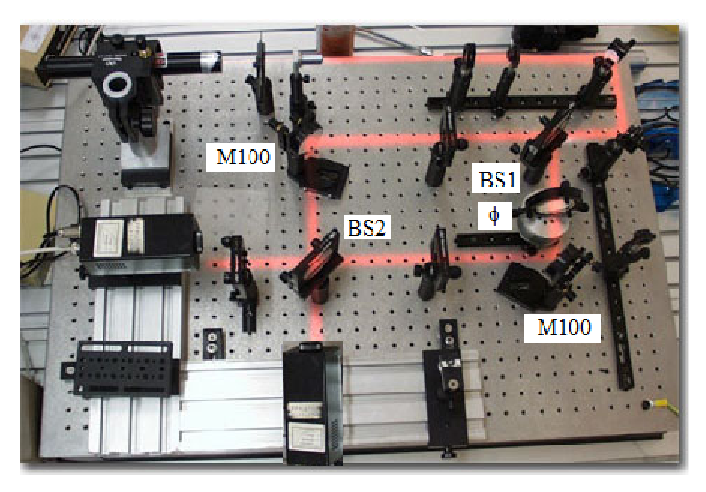
\includegraphics{graphics/MZPhaseImage.eps}%
\else
	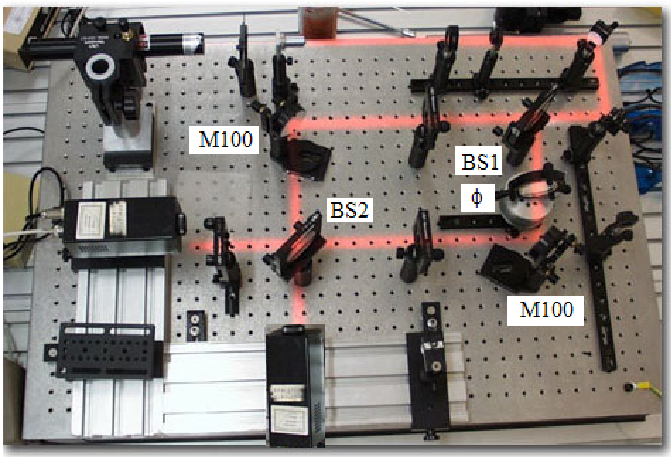
\includegraphics{graphics/MZPhaseImage.pdf}%
\fi
\end{minipage} \hfill
\begin{minipage}[c]{.30\linewidth}
\ifcase\msipdfoutput
	\includegraphics{graphics/MZPhas.eps}
\else
	\includegraphics{graphics/MZPhas.pdf}
\fi
\end{minipage}
\caption{Interféromètre de Mach-Zehnder déséquilibre (Image de laboratoire et
schéma de principe). La phase $\phi$ introduit une différence de marche ou de
longueur entre les deux bras. BS (Beam-Splitter) représente un miroir semi-
transparent. M100 est le miroir parfait.}%
\label{fig:MZPhase}%
\end{figure}

\colorbox[gray]{0.8}{
\parbox[c]{0.9\textwidth}{
\begin{definition}
Pour une expérience donnée, une \textbf{transition} est un ensemble
d'\textbf{états initiale et finale}.
\end{definition}
}}
\medskip

Dans l'expérience des fentes de Young, \emph{le passage d'un électron de la
source} $S$ \emph{pour arriver au détecteur à la position }$x$ est \textbf{une
transition}. Sur l'interféromètre de Mach-Zehnder déséquilibré, c'est par
exemple le passage d'un quanton du séparateur BS1 à un deux détecteurs.
L'objet de la théorie quantique est de prédire si cette transition a eu lieu
ou non.

On désigne par

\begin{itemize}
\item $\ket{x}$ le \textbf{vecteur d'état} qui représente \emph{le quanton qui
se propage dans la direction de }$x$;

\item $\ket{y}$ le \textbf{vecteur d'état} qui représente \emph{le quanton qui
se propage dans la direction de }$y$.
\end{itemize}

Les coefficients de réflexion $r$ et de transmission $t$ des quantons sur un
miroir semi-réfléchissant (BS) s'interprètent comme \emph{\textbf{les amplitudes
de probabilité (ou ondes de probabilité)} de réflexion et de transmission}.
Ainsi, la \textbf{probabilité} de trouver le quanton transmis par un BS unique
vaut alors $T=|t|^{2}$ et celle de le trouver réfléchi vaut $R=|r|^{2}$. Ces
probabilités doivent bien évidemment satisfaire à la \textbf{condition de
complétude}%
\begin{equation}
|t|^{2}+|r|^{2}=1.
\end{equation}
Puisque les BS de l'interféromètre de Mach-Zehnder sont équilibrés, on a, en
vertu de l'expérience MZ1,%
\begin{equation}
|t|^{2}=|r|^{2}=\frac{1}{2}\Rightarrow t=r=\frac{1}{\sqrt{2}}.
\end{equation}
Ainsi, l'action d'un BS est
\begin{equation}
\begin{cases}
\ket{x} \overset{BS}{\rightarrow}\ket{\psi_{x}} =t\ket{x}+ir\ket{y}
=\frac{1}{\sqrt{2}}(\ket{x} +i\ket{y}) \\
\ket{y} \overset{BS}{\rightarrow}\ket{\psi_{y}} =t\ket{y}+ir\ket{x}
=\frac{1}{\sqrt{2}}(\ket{y} +i\ket{x})
\end{cases}
\label{eq:ActionBS}
\end{equation}

\begin{enumerate}
\item Le facteur $i$ devant la partie réfléchie est due au fait que la
réflexion entraîne un déphasage de $\frac{\pi}{2}$ (entre le chemin incident
et le chemin réfléchi), soit un facteur de phase\footnote{En optique
ondulatoire, dans l'étude des interfaces, on suppose (hypothèse qui est
toujours formulée implicitement) que l'origine du temps sur le rayon réfléchi
est mesurée par le même observateur qui mesure le rayon incident.} $e^{i\pi
/2}=i$. Ce facteur donne un comportement symétrique aux entrées suivant $x$ et
suivant $y$.

\item $\ket{\psi_{x}}$ et $\ket{\psi_{y}}$ \emph{sont des \textbf{vecteurs
d'état} de même nature que} $\ket{x}$ et $\ket{y}$: ce sont des vecteurs
obtenu comme combinaison linéaires de deux vecteurs. Le vecteur $\ket{\psi_{x}}
$ (ou $\ket{\psi_{y}}$) décrit la \emph{\textbf{délocalisation}} du quanton
dans deux chemins indiscernables, due au BS.

\item Le principe physique correspondant à la possibilité de traiter les états
comme des vecteurs, et donc à pouvoir en prendre des combinaisons linéaires,
est appelé \textbf{principe de superposition des états.}
\end{enumerate}

Un miroir complètement réfléchissant (M100) réfléchi ou \emph{projette} un
quanton se déplaçant suivant un axe, sur l'axe orthogonal, avec une amplitude
de probabilité ou de projection $r^{\prime}$ de sorte que la probabilité de
trouver le quanton réfléchi M100 sur l'axe orthogonal est $|r^{\prime}|^{2}=1$:%
\begin{equation}%
\begin{array}
[c]{c}%
\ket{x} \overset{M100}{\rightarrow}i\ket{y}\\
\ket{y} \overset{M100}{\rightarrow}i\ket{x}
\end{array}
\end{equation}

La lame placée sur l'un des bras introduit une différence de chemin $\phi
=2\pi\frac{L}{\lambda}$ entre les deux bras qui se traduit un facteur de phase
$e^{i\phi}$, de module $1$, sur le vecteur représentant le chemin le plus
long:%
\begin{equation}
\ket{x} \overset{\phi}{\rightarrow}e^{i\phi}\ket{x}.
\end{equation}

\begin{figure}[tbh]
\centering
\ifcase\msipdfoutput
	\includegraphics{graphics/FormaMZ.eps}
\else
	\includegraphics{graphics/FormaMZ.pdf}
\fi
\caption{a) Dans un interféromètre alimenté par un champ classique,
l'intensité lumineuse $I(\varphi)$ en sortie oscille avec la différence de
phase $\varphi$ entre les deux chemins. b) Lorsqu'un photon unique est envoyé
dans l'interféromètre, la probabilité de photo-détection $P(\varphi)$ en
sortie varie avec $\varphi$ comme l'intensité qui serait obtenue pour un champ
classique. En traçant l'histogramme du nombre de photo-détections en fonction
de $\varphi$ lorsque l'expérience est répétée un grand nombre de fois, on
retrouve le système de franges attendu dans le cas classique [Après P.
Grangier \emph{et al. Europhys. Lett.,} \textbf{1}, 173 (1986)]}%
\label{fig:FormaMZ}%
\end{figure}

Ainsi, les amplitudes de probabilité ou ondes de probabilité des quatre
chemins possibles que peut emprunter le quanton envoyé suivant $x$ et détecter
après BS2 sont:%
\begin{equation}%
\begin{array}
[c]{ll}%
A(TR)=te^{i\phi}i(ir)=-tre^{i\phi} &
A(TT)=te^{i\phi}it=i|t|^{2}e^{i\phi} \\
A(RT)=(ir)it=-rt & A(RR)=(ir)i(ir)=-i|r|^{2}%
\end{array}
\label{eq:FactoAmpl1}%
\end{equation}
et les amplitudes de probabilité de détecter les quantons dans les sorties%
\begin{equation}%
\begin{array}
[c]{cc}%
x\ (TR\text{ ou }RT): & A(x)=A(TR)+A(RT)=-rt(1+e^{i\phi})=-\frac{1}%
{2}(1+e^{i\phi})\\
y\ (TT\text{ ou }RR): & A(y)=A(TT)+A(RR)=i(|t|^{2}e^{i\phi}-|r|^{2})
=\frac{i}{2}(e^{i\phi}-1)
\end{array}
\end{equation}
et les probabilités correspondantes (voir la figure \ref{fig:FormaMZ})%
\begin{equation}%
\begin{array}
[c]{c}%
\mathcal{P}(x)=|A(TR)+A(RT)|^{2}=|t|^{2}|r|^{2}|1+e^{i\phi}|^{2}%
=\frac{1}{2}(1+\cos\phi)=\cos^{2}\frac{\phi}{2}\\
\mathcal{P}(y)=|A(TT)+A(RR)|^{2}=|t|^{2}|r|^{2}|e^{i\phi}-1|^{2}%
=\frac{1}{2}(1-\cos\phi)=\sin^{2}\frac{\phi}{2}%
\end{array}
\end{equation}
On vérifie bien que
\begin{equation}
\mathcal{P}(x)+\mathcal{P}(y)=1.
\label{eq:RelCompl1}%
\end{equation}
Pour $\phi=2n\pi,$ $n\in\mathbb{N}$, tous les quantons sont détectés en $x$;
pour $\phi=(2n+1)\pi,$ $n\in\mathbb{N}$, tous les quantons sont détectés en
$y$.

\emph{\textbf{Il est donc clair que les quantons n'interfèrent jamais entre eux,
seuls interfèrent les champs ou amplitudes qui déterminent où et quand on peut
les trouver et avec quelle probabilité.}}

Cette interprétation que nous venons de faire est très générale:

\medskip
\colorbox[gray]{0.8}{
\parbox[c]{0.9\textwidth}{
\emph{il y a interférence chaque fois qu'un système physique peut prendre
plusieurs chemins distincts, pour évoluer vers un même état final, sans qu'il
soit possible, par quelque mesure que ce soit, de savoir quel chemin a été
emprunté (des chemins indiscernables). A chaque chemin est associée une
amplitude de probabilité $A$ et le carré du module de la somme de ces amplitudes
donne la probabilité $\mathcal{P}$ de trouver le système dans l'état final
considéré. Ainsi, dans un interféromètre à deux ondes comme un interféromètre de
Mach Zehnder, \textbf{ce ne sont pas les quantons qui interfèrent un à un; pour
chaque quanton, ce sont les amplitudes de probabilité associées aux deux chemins
qu'il peut prendre qui interfèrent}.}
}}

\subsection{Règles de calcul des amplitudes de probabilité}

Il apparaît que pour calculer les amplitudes de probabilités et les
probabilités quantiques, il faut définir des règles précises.

\colorbox[gray]{0.8}{
\parbox[c]{0.9\textwidth}{
\begin{definition}
\textbf{L'amplitude quantique}, qui détermine où et quand on peut trouver un
objet quantique et avec quelle probabilité, n'est définie que lorsque l'état
initial $\ket{i}$ et l'état final $\ket{f}$ du système quantique considéré sont
spécifiés de façon unique, c'est-à-dire décrivent exhaustivement le système tout
entier. Ces états $\ket{i}$ et $\ket{f}$ définissent une \textbf{transition
quantique.}
\end{definition}
}}

\begin{enumerate}
\item L'amplitude de probabilité de la transition $f\leftarrow i$ s'écrit
\begin{subequations}
\begin{equation}
A(f\leftarrow i)=\langle f\ket{i} ,
\end{equation}
et la \textbf{probabilité} correspondante s'écrit%
\begin{equation}
\mathcal{P}(f\leftarrow i)=|\langle f\ket{i}|^{2}.
\label{eq:BornRule}
\end{equation}
La relation (\ref{eq:BornRule}) est connue sous le nom de la \textbf{règle de
Born}.
\end{subequations}
\begin{itemize}
\item Dans le dispositif des fentes d'Young (DFY), on a%
\begin{equation}
A(x\leftarrow S)=\langle x\ket{S} .
\end{equation}

\item Dans l'interféromètre de Mach-Zehnder (IMZ), partant du quanton qui se
propage suivant $S_{x}$), on a la transition quantique menant au détecteur
suivant $x$ (TR ou RT) et la transition quantique menant au détecteur suivant
$y$ (TT ou RR). On a donc%
\begin{subequations}%
\begin{align}
A(x\leftarrow S_{x})=\langle x\ket{S_{x}}\\
A(y\leftarrow S_{x})=\langle y\ket{S_{x}}
\end{align}%

\end{subequations}%

\end{itemize}

\item Pour obtenir la probabilité $\mathcal{P}(f\leftarrow i)$ d'observer
l'état final $\ket{f}$, on additionne toutes les amplitudes quantiques
conduisant au résultat $\ket{f}$ en partant de $\ket{i}$:%
\begin{equation}
A(f\leftarrow i)=\sum_{n}A_{n}(f\leftarrow i),
\end{equation}
où les amplitudes $A_{n}$ correspondent aux divers chemins physiquement
indiscernables. D'où le principe suivant:

\colorbox[gray]{0.8}{
\parbox[c]{0.9\textwidth}{
\begin{principe}
\textbf{Superposition.} On somme les amplitudes quantiques correspondant à tous
les chemins indiscernables (par exemple TR ou RT; RR ou TT) ou à des états
finaux identiques.
\end{principe}
}}

\begin{itemize}
\item Dans DFY%
\begin{subequations}%
\begin{align}
A(x\leftarrow S_{x}) &=A_{F_1}(x\leftarrow S)+A_{F_2}(x\leftarrow S),\\
\langle x\ket{S}  &  =\langle x\ket{F_1}\langle F_1\ket{S} +\langle
x\ket{F_2}\langle F_2\ket{S}.
\label{eq:PSuperp}%
\end{align}%
\end{subequations}%

\item Dans IMZ,%
\begin{subequations}%
\label{eq:Amplixy}%
\begin{align}
A(x\leftarrow S_{x}) & =A(TR)(x\leftarrow S_{x})+A(RT)(x\leftarrow S_{x})\\
\langle x\ket{S_{x}} &  =\langle x\ket{R_2}\langle R_2\ket{M_{x}}\langle
M_{x}\ket{T_1}\langle T_1\ket{S_{x}}+\langle x\ket{T_2}\langle
T_2\ket{M_{y}}\langle M_{y}\ket{R_1}\langle R_1\ket{S_{x}}\\
A(y\leftarrow S_{x}) & =A(TT)(y\leftarrow S_{x})+A(RR)(y\leftarrow S_{x})\\
\langle y\ket{S_{x}} &  =\langle y\ket{T_2}\langle T_2\ket{M_{x}}\langle
M_{x}\ket{T_1}\langle T_1\ket{S_{x}}+\langle y\ket{R_2}\langle
R_2\ket{M_{y}}\langle M_{y}\ket{R_1}\langle R_1\ket{S_{x}}
\end{align}%
\end{subequations}%

\end{itemize}

Le fait d'ajouter les amplitudes de transition intermédiaires (l'électron
passe par $F_1$ ou $F_2$ par exemple) signifie qu'\textbf{on ne peut
attribuer au quanton une trajectoire bien définie}. Cependant, quelle que soit
la position $x$ du détecteur, l'amplitude $\langle x\ket{S}
$ est \textbf{complètement déterminée} par les amplitudes de transition
\textbf{vers} et \textbf{provenant }des deux fentes, celles-ci étant les
seules transitions possibles.

La superposition d'états quantiques ouvre la voie vers des applications très
sophistiquées comme

\begin{itemize}
\item la \textbf{cryptographie quantique} qui garantirait aux utilisateurs une
intimité absolue dans leur communication grâce au \textbf{qubit},
superposition des états $\alpha_{0}\left\vert 0\right\rangle +\alpha
_1\left\vert 1\right\rangle $ qui a une infinité de valeurs alors que le
\textbf{bit} classique ne peut prendre que deux valeurs, symbolisées par $0$
et $1$;

\item la \textbf{téléportation quantique} qui permet la transmission
d'information \emph{instantanée} sur des distances illimitées;

\item l'\textbf{ordinateur quantique} dont le temps de calcul sera
radicalement inférieur comparé à celle des ordinateurs classiques actuels. On
pense qu'en superposant les états quantiques qui réalisent des opérations
parallèles simultanément, les ordinateurs quantiques peuvent rompre des codes
de chiffrement et exercer d'autres miracles technologiques impossibles avec un
ordinateur classique.
\end{itemize}

Soulignons qu'à travers la superposition des états, la cryptographie
quantique repose sur le principe d'indétermination d'Heisenberg qui induit
que\emph{\ toute mesure perturbe nécessairement l'état des électrons }. Donc
toute tentative d'interception est détectée, même si on intercepte et que l'on
ré-injecte un électron dans le système après lecture.

\item Lorsqu'une transition peut se faire par des voies intermédiaires en
principe discernables, chacun de ces états peut être considéré comme final
pour une partie de la transition.

\colorbox[gray]{0.8}{
\parbox[c]{0.9\textwidth}{
\begin{principe}
\textbf{Addition des probabilités.} Lorsqu'on a pour un état initial plusieurs
états finaux différents ou disjoints, et donc plusieurs transitions quantiques,
la probabilité de transition vers l'ensemble de ces états est  la somme des
probabilités vers chacun de ces états:
\begin{equation}
\mathcal{P}(f\leftarrow i)=\sum_{n}\mathcal{P}(f_{n}\leftarrow i).
\end{equation}
\end{principe}
}}

Lorsque la somme des probabilité de transition est l'unité, on dit que ces
états forment un ensemble complet. C'est \emph{la propriété de
\textbf{complétude}} (voir l'Eq. (\ref{eq:RelCompl1})):%
\begin{equation}
\sum_{n}\mathcal{P}(f_{n}\leftarrow i)=1.
\end{equation}


\item Pour évaluer les amplitudes de l'Eq. (\ref{eq:FactoAmpl1}), nous avons
utilisé le principe suivant:

\colorbox[gray]{0.8}{
\parbox[c]{0.9\textwidth}{
\begin{principe}
\textbf{Factorisation séquentielle.} Lorsqu'une transition quantique peut se
décomposer en plusieurs \textbf{sous-transitions ou états intermédiaires},
l'amplitude de probabilité de la transition se factorise en produit des
amplitudes correspondant aux sous-transitions de la transitions:
\begin{equation}
A_{n}(f\leftarrow i)=A_{n}(f\leftarrow j)A_{n}(j\leftarrow k)\cdots
A_{n}(\ell\leftarrow i).\label{eq:PrinCFacto}\end{equation}
\end{principe}
}}

L'expression (\ref{eq:PrinCFacto}) s'énonce en lisant de droite à gauche,
puisque alors les différents états consécutifs occupés seront énoncés dans
l'ordre: état initial - état intermédiaire - état final.

Les sous-transitions ou états intermédiaires des divers transitions
indiscernables sont,

\begin{itemize}
\item dans DFY,%
\begin{subequations}%
\begin{align}
A_{F_1}(x\leftarrow S) =A_{F_1}(x\leftarrow F_1)A_{F_1}%
(F_1\leftarrow S)=\langle x\ket{F_1} \langle F_1\ket{S} ,\\
A_{F_2}(x\leftarrow S) =A_{F_2}(x\leftarrow F_2)A_{F_2}%
(F_2\leftarrow S)=\langle x\ket{F_2} \langle F_2\ket{S} ;
\end{align}%
\end{subequations}%

\item dans IMZ,
\begin{subequations}%
\begin{align}
A(TR)(x\leftarrow S_{x}) & =A(TR)(x\leftarrow R_2)A(TR)(R_2\leftarrow
M_{x})A(TR)(M_{x}\leftarrow T_1)A(TR)(T_1\leftarrow S_{x})\nonumber\\
&  =\langle x\ket{R_2}\langle R_2\ket{M_{x}}\langle M_{x}\ket{T_1}\langle
T_1\ket{S_{x}}\\
A(RT)(x\leftarrow S_{x}) & =A(RT)(x\leftarrow T_2)A(RT)(T_2\leftarrow
M_{y})A(RT)(M_{y}\leftarrow R_1)A(RT)(R_1\leftarrow S_{x})\nonumber\\
&  =\langle x\ket{T_2}\langle T_2\ket{M_{y}}\langle M_{y}\ket{R_1}\langle
R_1\ket{S_{x}}\\
A(TT)(y\leftarrow S_{x}) & =A(TT)(y\leftarrow T_2)A(TT)(T_2\leftarrow
M_{x})A(TT)(M_{x}\leftarrow T_1)A(TT)(T_1\leftarrow S_{x})\nonumber\\
&  =\langle y\ket{T_2}\langle T_2\ket{M_{x}}\langle M_{x}\ket{T_1}\langle
T_1\ket{S_{x}}\\
A(RR)(y\leftarrow S_{x}) & =A(RR)(y\leftarrow R_2)A(RR)(R_2\leftarrow
M_{y})A(RR)(M_{y}\leftarrow R_1)A(RR)(R_1\leftarrow S_{x})\nonumber\\
&  =\langle y\ket{R_2}\langle R_2\ket{M_{y}}\langle M_{y}\ket{R_1}\langle
R_1\ket{S_{x}}
\end{align}%
\end{subequations}%
où

\begin{enumerate}
\item $R_1$, $R_2$, $T_1$ et $T_2$ désignent les réflexions et les
transmissions sur $BS1$ et $BS2$;

\item $M_{x}$ et $M_{y}$ désignent respectivement les miroirs complètement
réfléchissant situés suivant $x$ et $y$ sur la figure (\ref{fig:MZPhase}).
\end{enumerate}
\end{itemize}

\item Dans (\ref{eq:PSuperp}), les termes $\langle x\ket{F_1}\langle F_2
\ket{S}$ et $\langle x\ket{F_2} \langle F_1\ket{S} $ sont implicitement
nuls. En effet, quelle est l'amplitude de transition pour qu'un électron parte
de $S$, passe par la fente $F_1$ (resp. $F_2$), sorte par la fente $F_2$
(resp. $F_1$)? La réponse à cette question devrait inclure la transition de
la fente $F_1$ (resp. $F_2$) à la fente $F_2$ (resp. $F_1$), i.e.,
l'amplitude $\langle F_1\ket{F_2} $ (resp.$\langle F_2\ket{F_1} $):%
\begin{equation}
\langle x\ket{F_1} \langle F_1\ket{F_2} \langle F_2\ket{S} \text{ ou
}\langle x\ket{F_2} \langle F_2\ket{F_1} \langle F_1\ket{S} .
\end{equation}
Cependant, on peut vérifier expérimentalement qu'on ne peut détecter un
électron qui entre par une fente et qui sort par une autre fente. Ainsi, les
transitions quantiques observées présentent la \emph{propriété de
\textbf{disjonction mutuelle}:}%
\begin{equation}
\langle F_1\ket{F_2} =\langle F_2\ket{F_1} =0.
\end{equation}
Signalons aussi que \emph{l'amplitude de transition (et la probabilité) entre
un état initial et un état final identiques est égale à l'unité:}%
\begin{subequations}%
\begin{align}
\langle F_1\ket{F_1} =\langle F_2\left\vert
F_2\right\rangle =1,\\
\mathcal{P}(i\leftarrow i)=1.
\end{align}%
\end{subequations}%

\item Si on considère un ensemble disjoint et complets d'états $f_{n}$, on
peut écrire%
\begin{subequations}%
\begin{align}
1  &  =\langle i\ket{i} =\sum_{n}\langle i\ket{f_{n}}\langle f_{n}\ket{i} \\
1  &  =\sum_{n}\mathcal{P}(f_{n}\leftarrow i)=\sum_{n}|\langle
f_{n}\ket{i}|^{2}%
\end{align}%
\end{subequations}%
Ces relations suggèrent que%
\begin{equation}
\langle f_{n}\ket{i} =\langle i\ket{f_{n}}^{\ast}.
\end{equation}
\colorbox[gray]{0.8}{
\parbox[c]{0.9\textwidth}{
\emph{D'où la \textbf{règle de conjugaison des amplitudes de probabilité
quantiques}: les amplitudes de probabilité quantiques de deux transitions
inverses l'une de l'autre sont complexes conjuguées}
\begin{equation}
\langle f\ket{i} =\langle i\ket{f}^{\ast }\text{ ou }A(f\leftarrow
i)=A^{\ast}(i\leftarrow f).\label{eq:ReglConjug}
\end{equation}
\emph{La conséquence immédiate est la \textbf{symétrie des probabilités:} les
probabilités des deux transitions quantiques inverses sont égales}
\begin{equation}
\mathcal{P}(f\leftarrow i)=\mathcal{P}(i\leftarrow f).
\end{equation}
}}
\medskip

Soulignons que
\begin{equation}
|\langle f\ket{i} |^{2}=\langle f\ket{i} ^{\ast}\langle f\ket{i}
=\langle i\ket{f}\langle f\ket{i} .
\end{equation}
Ainsi, en vertu de l'Eq. (\ref{eq:Amplixy}), on a%
\begin{subequations}%
\begin{align}
\mathcal{P}(x\leftarrow S_{x}) & =|\bra{x}S_{x}\rangle|^{2}=|A(TR)(x\leftarrow
S_{x})|^{2}+|A(RT)(x\leftarrow S_{x})|^{2}\nonumber\\
&  \left.  +A(TR)^{\ast}(x\leftarrow S_{x})A(RT)(x\leftarrow S_{x})
+A(RT)^{\ast}(x\leftarrow S_{x})A(TR)(x\leftarrow S_{x})\right. \\
\mathcal{P}(y\leftarrow S_{x}) & =|\bra{y}S_{x}\rangle|^{2}=|A(TT)(y\leftarrow
S_{x})|^{2}+|A(RR)(y\leftarrow S_{x})|^{2}\nonumber\\
&  \left.  +A(TT)^{\ast}(y\leftarrow S_{x})A(RR)(y\leftarrow S_{x}%
)+A(RR)^{\ast}(y\leftarrow S_{x})A(TT)(y\leftarrow S_{x})\right.
\end{align}%
\end{subequations}
Les produits $A(TR)^{\ast}(x\leftarrow S_{x})A(RT)(x\leftarrow S_{x})$,
$A(RT)^{\ast}(x\leftarrow S_{x})A(TR)(x\leftarrow S_{x})$, $A(TT)^{\ast
}(y\leftarrow S_{x})A(RR)(y\leftarrow S_{x})$ et $A(RR)^{\ast}(y\leftarrow
S_{x})A(TT)(y\leftarrow S_{x})$ sont les \textbf{termes d'interférences
quantiques.}

C'est donc à la superposition des amplitudes de probabilité et la règle de
conjugaison des amplitudes de probabilité quantiques qu'on doit les figures
d'interférence.

\medskip\colorbox[gray]{0.8}{
\parbox[c]{0.9\textwidth}{
\emph{Quand on dit que chaque quanton interfère avec lui-même, il
s'agit en fait d'interférences d'amplitudes de probabilité.}
}}
\end{enumerate}

Achevons ce chapitre, porte d'entrée dans le merveilleux monde quantique, en
notant que classiquement, on est habitué à un \emph{déterminisme} rigide et à la
relation de \emph{causalité}: quand on connaît les conditions initiales, on sait
parfaitement ce qui va se passer. En théorie quantique, ces certitudes sont
abandonnées. La possibilité de prévoir le comportement d'un système quantique
n'est qu'une prédictibilité probabiliste (un seul événement) et statistique
(grand nombre d'événements). L'objet quantique est en quelque sorte une
\emph{juxtaposition de possibles}: on parle d'\emph{indéterminisme}. On dit
aussi que \emph{Dieu joue au dés en théorie quantique}\footnote{Einstein n'a
jamais accepter le caractère probabiliste lié à la discontinuité des quanta
alors même qu'il avait prouvé en 1905 l'existence des atomes à partir d'une
interprétation probabiliste des fluctuations d'entropie dans le mouvement
brownien.}.

\medskip
\colorbox[gray]{0.8}{
\parbox[c]{0.9\textwidth}{
\emph{Tant que la mesure sur lui n'est pas faite, la grandeur censée quantifier
la propriété physique recherchée n'est pas strictement définie. Mais dès que
cette mesure est engagée, elle détruit la superposition quantique.}
}}

\subsection{Chat de Schrödinger}
\label{sec:EtatSuper}

Nous avons déjà annoncé la fin du chapitre, alors pourquoi cette section? Eh
bien, pour raconter une histoire au coin du feu!

C'est l'histoire du fameux du \textbf{paradoxe du chat de Schrödinger} dont
nous avons fait allusion à la \textbf{section \ref{sec:InterfMZ}}.

En effet, dans les années $1930$, ce célèbre physicien Autrichien avait, en
pensée, enfermé un chat dans une boîte en acier contenant un flacon de gaz
mortel, un compteur de radioactivité et un atome radioactif. Si le compteur
détecte de la radioactivité, un mécanisme casse le flacon, et le chat meurt. Le
compteur, appareil macroscopique, ne peut que mesurer l'un des deux états
classiques possibles de l'atome: \emph{désintégré} et \emph{non-désintégré}. On
suppose qu'après un temps $t_{1/2}$, l'atome se désintègre avec une probabilité
(quantique) $\frac{1}{2}$ (voir la figure \ref{fig:SchoedingerCat}). Tant
qu'aucune mesure n'est effectuée, cet atome se trouve dans un état superposé, à
la fois \emph{désintégré} et \emph{non-désintégré}. Par conséquent, tant que la
boîte reste fermée, le chat est dans un \textbf{état superposé}, \textbf{à la
fois mort et vivant}! Attention, le chat \textbf{n'est pas mort-vivant}, il est
soit mort, soit vivant, mais tant que la boîte n'est pas ouverte, notre
information sur son état est nécessairement constituée de ces deux possibilités.
C'est en l'observant que l'on constate que le chat est mort ou vivant. Donc, on
réduit le paquet d'ondes, transformant le chat de l'état superposé
$\frac{1}{\sqrt{2}}(\ket{vivant} + \ket{mort})$ à l'état $\ket{vivant}$ ou
$\ket{mort}$\footnote{En fait il n'y a pas paradoxe, puisque le principe de
superposition n'est valable que pour les états quantiques. Or le chat est
macroscopique.}.

\begin{figure}[ptbh]
\centering
\ifcase\msipdfoutput
  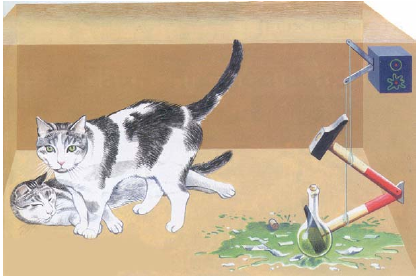
\includegraphics[scale=.8]{graphics/SchoedingerCat.eps}
\else
  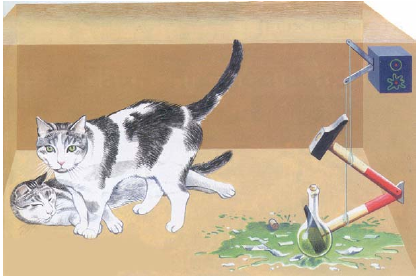
\includegraphics[scale=.8]{graphics/SchoedingerCat.png}
\fi
\caption{Le chat de Schrödinger dans la boîte d'acier. Tant que boîte reste
fermé, le chat est dans un état superposé mort et vivant.}
\label{fig:SchoedingerCat}
\end{figure}

Soulignons que depuis quelques années, la tendance en électronique quantique
est plutôt d'utiliser les mots \emph{chat de Schrödinger} d'une façon
différente, pour caractériser une superposition cohérente de possibilités
macroscopiquement distinctes. La cohérence du chat est évidemment une
condition suffisante pour qu'il soit dans un état flou à la Schrödinger (la
superposition cohérente sous entend nécessairement l'existence des deux
possibilités); mais elle n'est pas nécessaire.

Achevons cette histoire au coin du feu en nous demandant si le chat peut être
considéré comme un observateur: \emph{le chat peut-il avoir conscience d'être
mort ou vivant?} Le chat ne peut avoir conscience par définition que d'être
vivant. Cependant, cela ne l'empêche pas de constituer un observateur
acceptable: vivant, il peut laisser dans la boîte des traces de son état, mort,
il laisse d'autres types de traces, de sorte que la \emph{mesure} de son état
vivant ou mort serait également l'inscription rétroactive (en remontant le temps
!) des traces laissées.
\bigskip

\emph{Wolai!! Effectuer la mesure dans le monde quantique est une histoire
compliquée!!}

\begin{remark}

\begin{small}
Bien que le dispositif de Schrödinger soit, il a l'intérêt de mettre en
évidence, qu'en principe au moins, l'étrangeté quantique des systèmes
microscopiques se communique aux systèmes macroscopiques. Et il pose une
question de fond: \emph{pourquoi les gens ne voient-ils que des chats soit
vivants, soit morts et pas de chats morts-vivants?}

D'après la vision actuelle, si le monde semble si bien décrit par la physique
classique, c'est parce que les interactions complexes d'un objet avec son
environnement font très vite disparaître les particularités quantiques.
L'information relative à l'état de santé d'un chat, par exemple, gagne
rapidement son environnement sous la forme de photons et d'échanges de chaleur.
Chaque phénomène quantique peut impliquer des états superposés du système en jeu
(mort ou vivant), mais ces états tendent à disparaître. La fuite permanente
d'information vers l'environnement est le mécanisme essentiel par lequel les
états quantiques de superposition se détruisent, processus nommé
\textbf{décohérence}. Les gros systèmes sont davantage sujets à la décohérence
que les petits, tout simplement parce qu'ils laissent échapper plus
d'informations. C'est pourquoi les physiciens tendent à associer la théorie
quantique au monde microscopique. Dans de nombreux cas, toutefois, la perte
d'information par un gros système peut être ralentie ou stoppée, ce qui met
alors en évidence l'omniprésence des phénomènes quantiques.
\end{small}

\end{remark}

\newpage

\section{Exercices et problèmes}

\subsection{Interféromètre de Mach-Zehnder à deux lames}
\begin{figure}[ptbh]
\centering
	\ifcase\msipdfoutput
		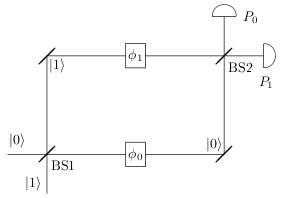
\includegraphics[scale=.8]{graphics/InterferometreEkert.eps}%
	\else
		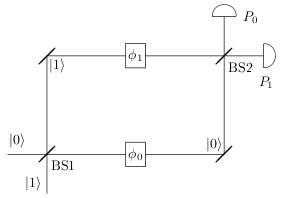
\includegraphics[scale=.8]{graphics/InterferometreEkert.jpg}%
	\fi
\caption{MZ à deux lames.}
\label{fig:MZ2Lames}
\end{figure}

On considère l'interféromètre de la figure \ref{fig:MZ2Lames}. Le quanton qui y
pénètre est soit dans l'état $ \ket{0}$, soit dans l'état $\ket{1}$. Quelles
sont les probabilités $\mathcal{P}_{0}$ et $\mathcal{P}_1$ ce quanton aux
détecteurs $D_{0}$ et $D_1$?

\subsection{Amplitudes de probabilité de transition}

\begin{figure}[ptbh]
\centering
\begin{minipage}[c]{.6\linewidth}
	\ifcase\msipdfoutput
		\includegraphics[scale=.8]{graphics/DispoYoung.eps}%
	\else
		\includegraphics[scale=.8]{graphics/DispoYoung.pdf}%
	\fi
\caption{Dispositif des fentes d'Young. Les fentes $F_1$ et $F_2$ sont à
la même distance $r_{0}$ de la source $S$.}%
\label{fig:DispoYoung}%
	\end{minipage} \hfill\begin{minipage}[c]{.38\linewidth}
	\ifcase\msipdfoutput
		\includegraphics{graphics/FigInterfPhotons.eps}%
	\else
		\includegraphics[scale=.9]{graphics/FigInterfPhotons.pdf}%
	\fi
\caption{Figure d'interférences photon par photon [École Normale Supérieure de
Cachan (France, 2005)].}%
\label{fig:FigInterfPhotons}%
\end{minipage}
\end{figure}

Pour un photon d'énergie bien définie, $E=\hbar\omega$, l'amplitude de
probabilité de transition d'un point $A$ à un point $B$ est donnée par:%
\begin{equation}
\langle B\ket{A}=\varphi(AB)e^{-i\omega t},
\label{eq:AmplAB}%
\end{equation}
où $t$ est le temps de parcours et $\varphi(AB)$ est une fonction qui dépend
uniquement de la distance entre les points $A$ et $B$. Dans le cas où la
divergence d'un faisceau de lumière peut être négligée tous les photons
partant de $A$ arrivent en $B$. La probabilité de transition pour un photon
est égale à l'unité. L'amplitude de probabilité est alors de la forme:%
\begin{equation}
\langle B\ket{A}=e^{i\alpha}e^{-i\omega t},
\end{equation}
L'amplitude étant indéterminée à un facteur de phase près on peut poser
$\alpha=0$.

Grâce à un dispositif spécial, la source $S$ ne produit que des photons
uniques qui passent soit par $F_1$, soit par $F_2$ et peuvent être
détectés au point $X$ (voir la figure \ref{fig:DispoYoung}). Il existe deux
chemins en principe indiscernables.

\begin{enumerate}
\item Appliquer le principe de superposition pour exprimer l'amplitude de
probabilité $\ket{\psi} =\langle X\ket{S}$ du photon détecté au point $X$.
Expliciter cette expression à l'aide du principe de factorisation séquentielle.
En déduire l'expression de la probabilité $\mathcal{P}(X\leftarrow S)$ pour
qu'un photon émis par la source $S$ arrive en $X$ en passant par l'une ou
l'autre fente en faisant apparaître explicitement les termes
d'\emph{interférences quantiques}, en supposant que les amplitudes de
probabilité de transition de la source $S$ aux fentes $F_1$ et $F_2$ sont
les mêmes.

\item Soient $t_{0}$ le temps de parcours de la source à l'une des fentes,
$t_1$ le temps de parcours de la fente $F_1$ au point $X$, $t_2$ le
temps de parcours de la fente $F_2$ au point $X$. Exprimer, en vertu de
l'Eq. (\ref{eq:AmplAB}), chaque amplitude de probabilité de transition
intermédiaire en fonction $r_{i}$ et $t_{i}$ et en déduire l'expression de
$\ket{\psi} $.

\item Aux grandes distances, c'est-à-dire lorsque $r_1$ et $r_2$ sont
beaucoup plus grands que la distance entre des fentes les amplitudes
$\varphi(r_1)$ et $\varphi(r_2)$ sont à peu près égales et on peut écrire
$\varphi(r_1)=\varphi(r_2)=C^{\prime}$. Montrer que la probabilité pour
qu'un photon émis par la source $S$ arrive en $X$ en passant par l'une ou
l'autre fente est de la forme%
\begin{equation}
\mathcal{P}(X\leftarrow S)=2|C|^{2}\left[1+\cos\frac{\omega}{c}(r_2-r_1)
\right].
\end{equation}

\item Pour quelles valeurs de la différence de marche $r_2-r_1$, en
fonction de $\lambda$, a-t-on les franges brillantes et des franges sombres
(voir la figure (\ref{fig:FigInterfPhotons}))?
\end{enumerate}

\subsection{Chat de Schrödinger}

Nous reprenons dans cette exercice, la célèbre expérience de pensée de
Schrödinger en considérant un chat enfermé dans une boîte avec un poison
(substance radioactive) qui va déclencher la mort du chat à un moment ou un
autre. Classiquement, le chat est soit mort, soit vivant. Quantiquement, on
dit que le chat est dans une \emph{superposition d'états mort ou vivant.}

\begin{enumerate}
\item Quelle base conceptuelle de la physique classique se trouve remise en
cause par cette expérience?

\item On se place dans la situation quantique. On désigne l'état mort et
l'état vivant par les kets respectifs $\ket{m}$ et $\ket{v}$.

\begin{enumerate}
\item Exprimer dans la base $\{\ket{m},\ket{v}\} $ un état quelconque
$\ket{\psi}$ du chat.

\item Quelle condition doit être remplie pour que cet état traduise une onde
de probabilité?

\item Quels sont les deux états \emph{limites}? Quand les obtient-on?

\item Soit $t_1$ le temps au bout duquel le chat a une chance sur deux d'être
vivant et $t_2$ celui au bout duquel il a une chance sur quatre d'être vivant.
Exprimer les états $\ket{\psi_1}$ et $\ket{\psi_2}$ du chat correspondant à
ces instants.
\end{enumerate}
\end{enumerate}

